\newpage
\section{Lexical Analysis}
To translate a program from one language into another, a compiler first pull it apart and understand its structure and meaning, then put it together in a different way.

\begin{itemize}
    \item The front end(前端): performs analysis
    \item The back end(后端): performs synthesis
\end{itemize}

The analysis is usually broken up into:
\begin{enumerate}
    \item Lexical analysis
    \item Syntax analysis
    \item Semantic analysis
\end{enumerate}

Task of the lexical analyzer:
\begin{enumerate}
    \item Taking a stream of characters
    \item Produces a stream of tokens
    \item Discarding white space and comments
\end{enumerate}

\subsection{Lexical Token}
\subsubsection{A lexical token}
\begin{itemize}
    \item A sequence of characters
    \item A unit in the grammar of a programming language
\end{itemize}

\subsubsection{Token types}
Classification of lexical tokens: A finite set of token types.
\begin{figure}[!htb]
    \centering
    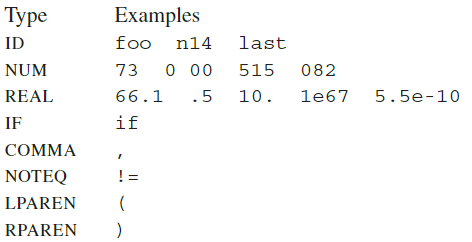
\includegraphics[width=0.42\textwidth]{pic/CP2/Token types}
    \caption{Token types}
\end{figure}

\subsubsection{Non-Tokens}
\begin{figure}[!htb]
    \centering
    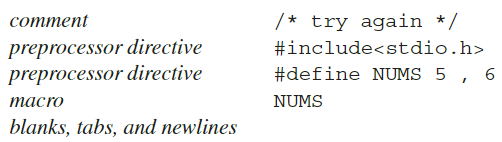
\includegraphics[width=0.42\textwidth]{pic/CP2/Non-Tokens}
    \caption{Non-Tokens}
\end{figure}
The preprocessor deletes the non-tokens.

\subsubsection{An example}
\begin{minted}{c}
float match0(char *s){ /* find a zero */
    if (!strncmp(s, "0.0", 3))
        return 0.;
}
\end{minted}

\begin{minted}{text}
FLOAT ID(match0) LPAREN CHAR STAR ID(s) RPAREN LBRACE 
IF LPAREN BANG ID(strncmp) LPAREN ID(s) COMMA STRING(0.0) COMMA NUM(3) RPAREN RPAREN 
RETURN REAL(0.0) SEMI 
RBRACE EOF
\end{minted}



\subsubsection{An ad hoc lexer}
Any reasonable programming language can be used to implement it. (人和代码有一个能跑就行)

\subsubsection{A simpler and more readable lexical analyzers}
\begin{itemize}
    \item Regular expressions: Specify lexical tokens
    \item Deterministic finite automata: Implementing lexers
    \item Mathematics: Connecting the above two
\end{itemize}

\subsection{Regular Expression}
\subsubsection{Some Concepts}
\begin{itemize}
    \item A language is a set of strings
    \item A string is a finite sequence of symbols (string 没有被赋予意义)
    \item A symbol is taken from a finite alphabet
\end{itemize}

\subsubsection{The notation of regular expressions}
% \begin{itemize}
%     \item Symbol: a
%     \item Alternation: A vertical bar $|$
%     \item Concatenation: operator $\cdot$
%     \item Epsilon: $\epsilon$
%     \item Repetition: ${}^*$
%     \subitem Given a regular expression $M$, its Kleene closure is $M^*$.
%     \subitem A string is in $M^*$ if it is the concatenation of zero or more strings, all of which are in M.
% \end{itemize}

\begin{figure}[!htb]
    \centering
    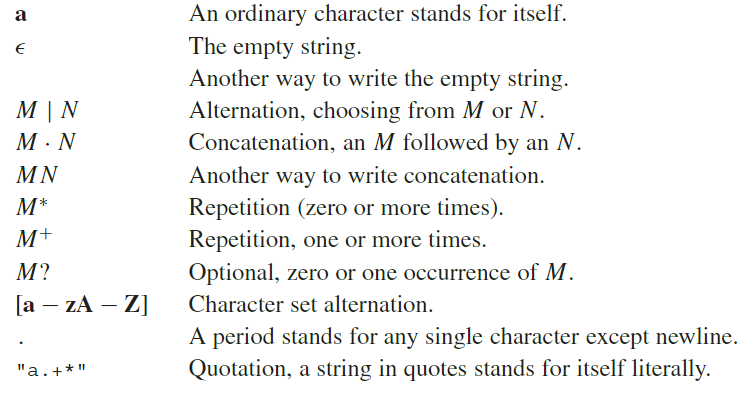
\includegraphics[width=0.42\textwidth]{pic/CP2/Regular expression notation}
    \caption{Regular expression notation}
\end{figure}

\begin{figure}[!htb]
    \centering
    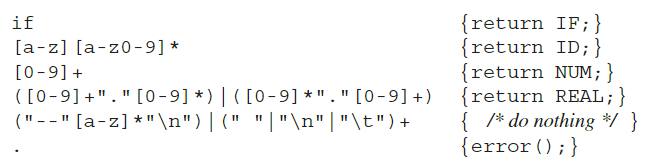
\includegraphics[width=0.42\textwidth]{pic/CP2/Regular expressions for some tokens}
    \caption{Regular expressions for some tokens}
\end{figure}

优先级: ${}^*> \cdot > ||$.

\begin{example}\quad

    \begin{enumerate}
        \item $(0|1)*\cdot0$
        \subitem Binary numbers that are multiples of two
    \end{enumerate}
\end{example}

\subsubsection{Two important disambiguation rules}
These rules are a bit ambiguous.

\begin{enumerate}
    \item Longest match
    \subitem The longest initial substring of the input that can match any regular expression is taken as the next token.
    \item Rule priority
    \subitem The first regular expression that can match determines its token-type
\end{enumerate}

\subsection{Finite Automata}
\subsubsection{A finite automaton}
\begin{definition}[A finite automaton]\quad 
    \begin{itemize}
        \item A finite set of states;
        \item Edges lead from one state to another, and each edge is labeled with a symbol ;
        \item One state is the start state, and certain of the states are distinguished as final states.
    \end{itemize}
\end{definition}

\begin{figure}[!htb]
    \centering
    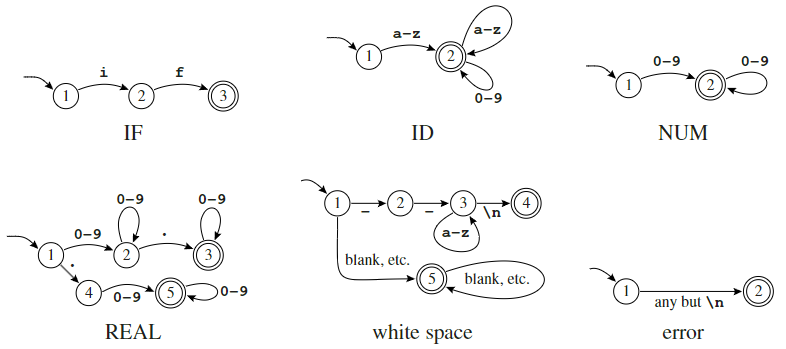
\includegraphics[width=0.42\textwidth]{pic/CP2/Finite automata for lexical tokens.}
    \caption{Finite automata for lexical tokens.}
\end{figure}

\subsubsection{Deterministic Finite Automaton (DFA)}
A DFA accepts or rejects a string as follows: TLDR. 

看计算理论 II.1-6.

\subsubsection{Combined finite automaton}
Using ad hoc method.

\begin{figure}[!htb]
    \centering
    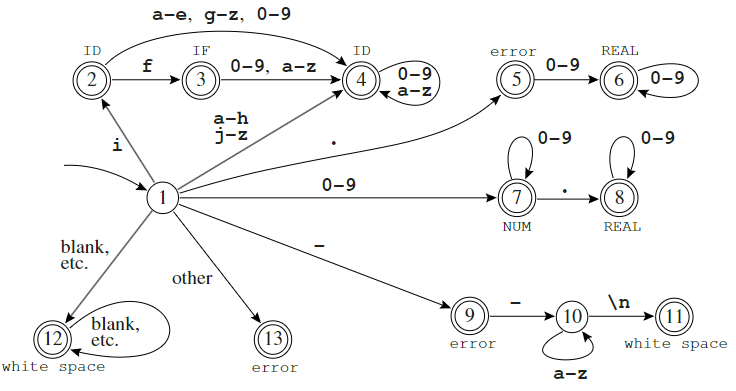
\includegraphics[width=0.42\textwidth]{pic/CP2/Combined finite automaton}
    \caption{Combined finite automaton}
    \label{fig:CDFA}
\end{figure}

\subsubsection{A transition matrix}
Encoding \textbf{Figure} \ref{fig:CDFA}

\subsection{Nondeterministic Finite Automata}
\subsubsection{NFA}
A NFA: 
\begin{itemize}
    \item Have to choose one from the edges to follow out of a state
    \item Have special edges labeled with $\epsilon$
\end{itemize}

\subsubsection{From a RE to an NFA}
The conversion algorithm: (计算理论 III.2 上说这个转换是 naive 的)
\begin{enumerate}
    \item Turning each regular expression into an NFA with a tail (start edge) and a head (ending state).
    \item The rules for translating
\end{enumerate}

\subsubsection{From an NFA to a DFA}
To avoid guesses by trying every possibility at once.

这个计算理论有, II.13.

\subsubsection{The equivalent states}
略
\subsection{Lex: A Lexical Analyzer Generator}
看书